\documentclass{article}
%\usepackage[brazil]{babel}
\usepackage[utf8]{inputenc}
\usepackage{geometry}
\usepackage{tikz}
\usepackage{amsmath}
\usepackage{amssymb}
\usepackage{graphicx,xcolor,lipsum,multicol,caption}
\usetikzlibrary{arrows.meta,
	chains,
	fit,
	positioning,
	quotes}

\begin{document}
	\begin{center}
	\section*{\normalsize  Catálogo Gaia de estrelas até $23.0$ parsecs do Sol\\ \small Correções}
	\end{center}
	\vspace{50pt}
	
	\begin{enumerate}
		
		\item O diagrama \textcolor{blue}{$M(Vt)$ versus $BT-VT$} do sub catálogo Gaia $\cap$ Hipparcos tem $2$ estrelas a menos. O valor anterior era de $556$ estrelas, o valor correto é $554$ estrelas.
		
		\begin{multicols}{2}
			\centering
			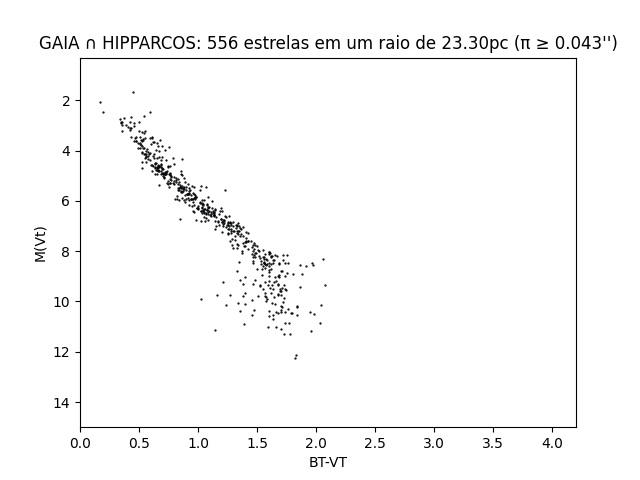
\includegraphics[width=.98\linewidth]{gaia_intersection_hipparcos_mvt_versus_bt_minus_vt_plx_greater_than_0.png}
			\captionof*{figure}{diagrama antigo}
			\columnbreak
			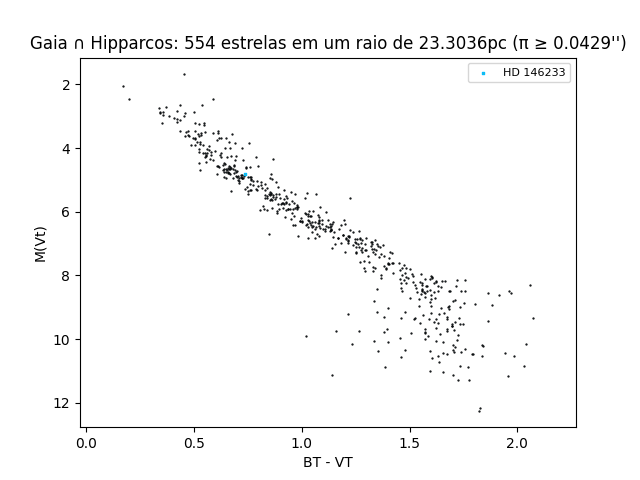
\includegraphics[width=.98\linewidth]{Gaia_intersection_Hipparcos_MVt_versus_BT_minus_VT.png}
			\captionof*{figure}{diagrama atual}
		\end{multicols}
	
    	As duas estrelas que saíram do diagrama foram as seguintes:
	
		\begin{table}[h]
			\centering
			\begin{tabular}{|l|l|l|l|l|l|l|l|l|l|l|l|l|}
				\hline
				\tiny{designation}  
				& \tiny{HIP}   
				& \tiny{HD} 
				& \tiny{parallax}   
				& \tiny{Plx}        
				& \tiny{BTmag}             
				& \tiny{VTmag}          
				& \tiny{M(Vt)}  
				& \tiny{B-V}
				& \tiny{BT-VT} \\ \hline
				\tiny{3023711269067191296} 
				& \tiny{27435} 
				& \tiny{38858} 
				& \tiny{65.74459508507027} 
				& \tiny{64.25}  
				& \tiny{\textcolor{red}{NULL}} 
				& \tiny{6.39} 
				& \tiny{5.429365660016661} 
				& \tiny{0.639}
				& \tiny{\textcolor{red}{NULL}}  \\ \hline
				\tiny{3837697972130323456} 
				& \tiny{46509} 
				& \tiny{81997}
				& \tiny{54.9186971699019} 
				& \tiny{58.48}  
				& \tiny{\textcolor{red}{NULL}} 
				& \tiny{4.922} 
				& \tiny{3.757036819749022} 
				& \tiny{0.411}
				& \tiny{\textcolor{red}{NULL}}  \\ \hline
			\end{tabular}
		\end{table}
	
		A estrela $HIP \;\; 27435$ não tem $BTmag$ e, por isso, também não tem $BT-VT$. 
		
		O que estava sendo feito antes era $BTmag = 0$ e $BT-VT = -6.39$. 
		
		Com isso, estava sendo plotado o ponto com coordenadas \textcolor{blue}{$(-6.39\;,\;5.429365660016661)$}. 
		
		O mesmo aconteceu para a estrela $HIP \;\; 46509$, para a qual estava sendo plotado o ponto \textcolor{blue}{$(-4.922\;,\;3.757036819749022)$}. 
		
		Observações:
		
		\begin{enumerate}
			\item Estes pontos não aparecem no diagrama antigo porque as dimensões estavam fixas, isto é, não estavam sendo considerados os valores plotados para definir as dimensões da imagem. Apesar destes pontos não aparecerem, estas duas estrelas estavam sendo contabilizadas para o valor $556$ que aparece no título da figura do diagrama antigo.
			
			\item As dimensões do diagrama atual estão sendo feitas de forma mais automática. Identificamos o menor e o maior valor de BT-VT para configurar a dimensão horizontal da figura. O mesmo é feito para o eixo y.
		\end{enumerate}

	
		\newpage
	
		\item O diagrama \textcolor{blue}{$M(Vt)$ versus $BT-VT$} do sub catálogo Hipparcos $-$ Gaia tem $2$ estrelas a menos. O valor anterior era de $635$ estrelas, o valor correto é $633$ estrelas. 
		
		\begin{multicols}{2}
			\centering
			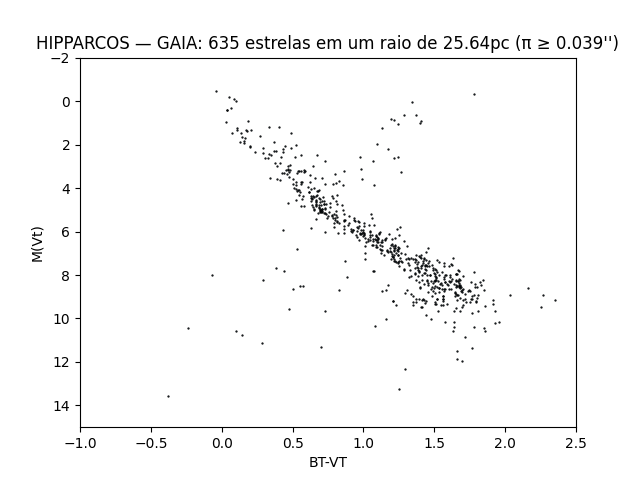
\includegraphics[width=.98\linewidth]{hipparcos_minus_gaia_mvt_versus_bt_minus_vt_plx_greater_than_or_iqual_to_0.039.png}
			\captionof*{figure}{diagrama antigo}
			\columnbreak
			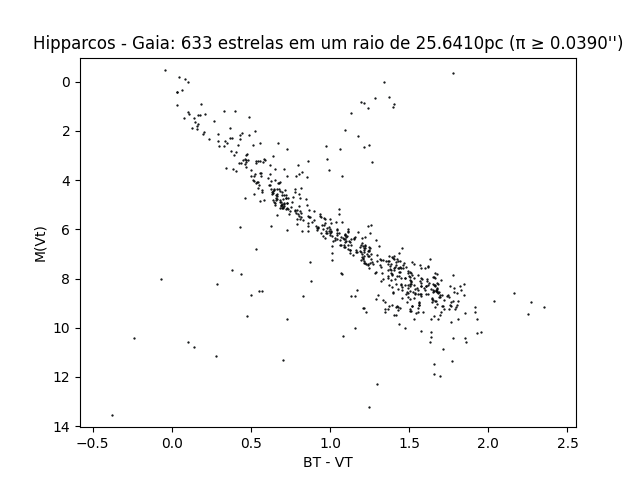
\includegraphics[width=.98\linewidth]{Hipparcos_minus_Gaia_MVt_versus_BT_minus_VT.png}
			\captionof*{figure}{diagrama atual}
		\end{multicols}
	
    	As duas estrelas que saíram do diagrama foram as seguintes:
	
		\begin{table}[h]
			\centering
			\begin{tabular}{|l|l|l|l|l|l|l|l|l|l|l|l|}
				\hline
				  \tiny{HIP}  
				& \tiny{HD}   
				& \tiny{Vmag} 
				& \tiny{Plx}   
				& \tiny{BTmag} 
				& \tiny{VTmag}        
				& \tiny{M(Vt)}             
				& \tiny{M(Vt) error}          
				& \tiny{B-V}  
				& \tiny{BT-VT} \\ \hline
				  \tiny{5896} 
				& \tiny{7788} 
				& \tiny{4.25} 
				& \tiny{48.94} 
				& \tiny{\textcolor{red}{NULL}}  
				& \tiny{8.439} 
				& \tiny{6.887319825078853} 
				& \tiny{0.023517069308228944} 
				& \tiny{0.48}
				& \tiny{\textcolor{red}{NULL}}  \\ \hline
				  \tiny{35296} 
				& \tiny{57095} 
				& \tiny{6.7} 
				& \tiny{67.69} 
				& \tiny{\textcolor{red}{NULL}}  
				& \tiny{7.437} 
				& \tiny{6.589622570486292} 
				& \tiny{0.027589995004595913} 
				& \tiny{0.975}
				& \tiny{\textcolor{red}{NULL}}  \\ \hline
			\end{tabular}
		\end{table}
	
		A estrela $HIP \;\; 5896$ não tem $BTmag$ e, por isso, também não tem $BT-VT$. 

		O que estava sendo feito antes era $BTmag = 0$ e $BT-VT = -8.439$. 
		
		Com isso, estava sendo plotado o ponto com coordenadas \textcolor{blue}{$(-8.439\;,\;6.887319825078853)$}. 
		
		O mesmo aconteceu para a estrela $HIP \;\; 35296$, para a qual estava sendo plotado o ponto \textcolor{blue}{$(-7.437\;,\;6.589622570486292)$}. 
		
		Observações:
		
		\begin{enumerate}
			\item Estes pontos não aparecem no diagrama antigo porque as dimensões estavam fixas, isto é, não estavam sendo considerados os valores plotados para definir as dimensões da imagem. Apesar destes pontos não aparecerem, estas duas estrelas estavam sendo contabilizadas para o valor $635$ que aparece no título da figura do diagrama antigo.
			
			\item As dimensões do diagrama atual estão sendo feitas de forma mais automática. Identificamos o menor e o maior valor de BT-VT para configurar a dimensão horizontal da figura. O mesmo é feito para o eixo y.
		\end{enumerate}

		\newpage
		
		\item No Diagrama \textcolor{blue}{$M(V)$ versus $B-V$} do sub catálogo Hipparcos $-$ Gaia, tem uma estrela no canto inferior direito que não estava aparecendo no diagrama anterior. Isto porque o tamanho da imagem não estava ajustado.

		\begin{multicols}{2}
			\centering
			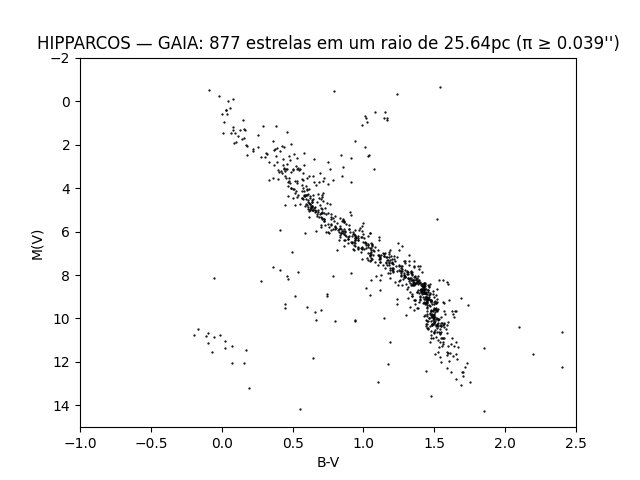
\includegraphics[width=.98\linewidth]{hipparcos_minus_gaia_mv_versus_b_minus_v_plx_greater_than_or_iqual_to_0.039.png}
			\captionof*{figure}{diagrama antigo}
			\columnbreak
			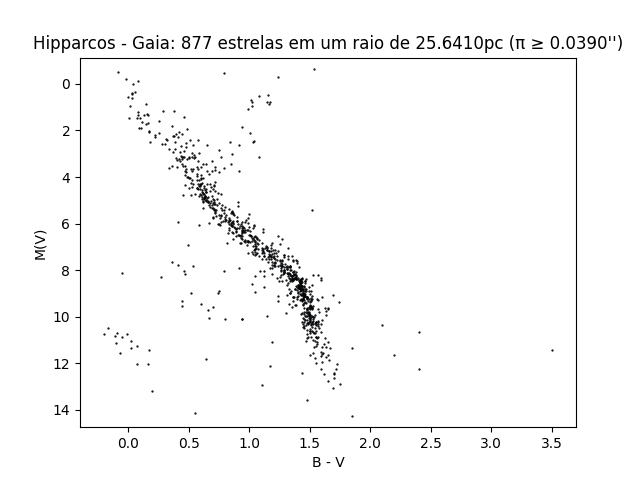
\includegraphics[width=.98\linewidth]{Hipparcos_minus_Gaia_MV_versus_B_minus_V.png}
			\captionof*{figure}{diagrama atual}
		\end{multicols}
	
    	A estrela que não estava aparecendo no diagrama antigo é a seguinte:

		\begin{table}[h]
			\centering
			\begin{tabular}{|l|l|l|l|l|l|l|l|l|l|l|l|}
				\hline
				\tiny{HIP}  
				& \tiny{HD}   
				& \tiny{Vmag} 
				& \tiny{Plx}   
				& \tiny{BTmag} 
				& \tiny{VTmag}        
				& \tiny{M(V)}        
				& \tiny{M(Vt)}             
				& \tiny{M(Vt) error}          
				& \tiny{B-V}  
				& \tiny{BT-VT} \\ \hline
				\tiny{50798} 
				& \tiny{\textcolor{black}{NULL}} 
				& \tiny{11.49} 
				& \tiny{98.17} 
				& \tiny{\textcolor{black}{NULL}}  
				& \tiny{\textcolor{black}{NULL}} 
				& \tiny{11.449893954972916} 
				& \tiny{\textcolor{black}{NULL}} 
				& \tiny{\textcolor{black}{NULL}} 
				& \tiny{3.5}
				& \tiny{\textcolor{black}{NULL}}  \\ \hline
			\end{tabular}
		\end{table}
		
		\newpage
		
		\item A quantidade de estrelas que possuem tanto designação Gaia quanto designação Hipparcos é \textcolor{blue}{$755$}. O valor anterior de $744$ foi encontrado considerando-se a distância limite de $25.64$ parsecs do catálogo $2$.
		
	    As $11$ estrelas adicionais se encaixam em alguma das seguintes situações:
		
		\begin{itemize}
			\item Possuem paralaxe no Hipparcos menor do que $0.039$\textquotesingle \textquotesingle
			\item Não possuem valor de paralaxe no Hipparcos
		\end{itemize}
	
		Abaixo, está a tabela com algumas informações das $11$ estrelas adicionais:

		\hspace{20pt}		

		\begin{figure}[h]
			\centering
			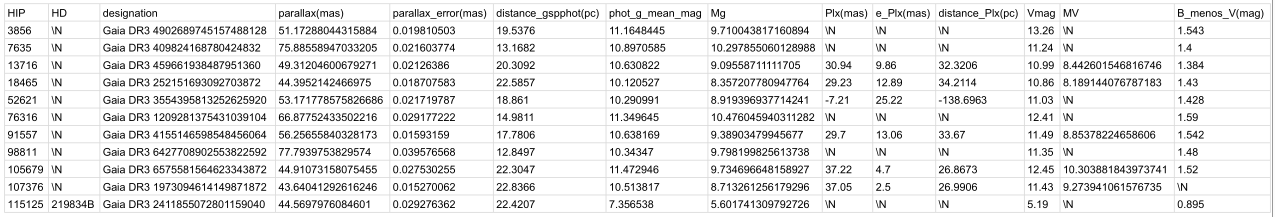
\includegraphics[width=.98\linewidth]{dados_onze_estrelas.png}
			\caption*{informações das $11$ estrelas adicionais}
		\end{figure}


		
	\end{enumerate}
	
	
\end{document}